% !TeX program = xelatex
\documentclass[12pt,a4paper]{article}
% bidi's table adaptation expects the pre-2026 array implementation.
\RequirePackage{array}[=2024-06-01]
% !TeX root = ../2/main.tex
\usepackage[a4paper,margin=25mm,headheight=16pt]{geometry}
\usepackage{amsmath,amssymb}
\usepackage{graphicx}
\usepackage{booktabs}
\usepackage{tabularx}
\usepackage{siunitx}
\usepackage{tikz}
\usepackage{circuitikz}
\usepackage[unicode,hidelinks]{hyperref}
\usepackage{xepersian}
% Only the regular B Nazanin file is installed; synthesize bold explicitly.
\settextfont[Path=C:/Windows/Fonts/,AutoFakeBold=2,AutoFakeSlant=0.2]{B-NAZANIN.TTF}
% B Nazanin lacks U+066A (Arabic percent), required by xepersian's digit setup.
% Arial covers the complete required digit/punctuation set; Persian prose remains B Nazanin.
\setdigitfont[Path=C:/Windows/Fonts/,BoldFont=arialbd.ttf,ItalicFont=ariali.ttf,BoldItalicFont=arialbi.ttf]{arial.ttf}
\setmathdigitfont[Path=C:/Windows/Fonts/,BoldFont=arialbd.ttf,ItalicFont=ariali.ttf,BoldItalicFont=arialbi.ttf]{arial.ttf}
\setlatintextfont{TeX Gyre Termes}
% B Nazanin does not contain the default itemize bullet and dash glyphs.
\renewcommand{\labelitemi}{\(\bullet\)}
\renewcommand{\labelitemii}{\(\circ\)}
\renewcommand{\labelitemiii}{\(\diamond\)}
\setlength{\parindent}{0pt}
\setlength{\parskip}{0.5em}
\linespread{1.25}
\newcommand{\exercise}[1]{\section*{تمرین #1}}
% !TeX root = ../2/main.tex
% Shared title page for every assignment.
% Change only \AssignmentNumber and \AssignmentDate in each main document.

\newcommand{\AssignmentNumber}[1]{\gdef\assignmentnumber{#1}}
\newcommand{\AssignmentDate}[1]{\gdef\assignmentdate{#1}}

\newcommand{\assignmentnumber}{---}
\newcommand{\assignmentdate}{---}

% Stable course metadata
\newcommand{\universityname}{دانشگاه صنعتی امیرکبیر}
\newcommand{\universityalias}{پلی‌تکنیک تهران}
\newcommand{\facultyname}{دانشکده مهندسی کامپیوتر}
\newcommand{\coursename}{طراحی مدارهای مجتمع پرتراکم پیشرفته}
\newcommand{\studentname}{محمد خلیلی اصل}
\newcommand{\instructorname}{دکتر مهدی صدیقی}

\newcommand{\MakeAssignmentCover}{%
  \begin{titlepage}
    \thispagestyle{empty}
    \centering
    \linespread{1}\selectfont

    \vspace*{0mm}
    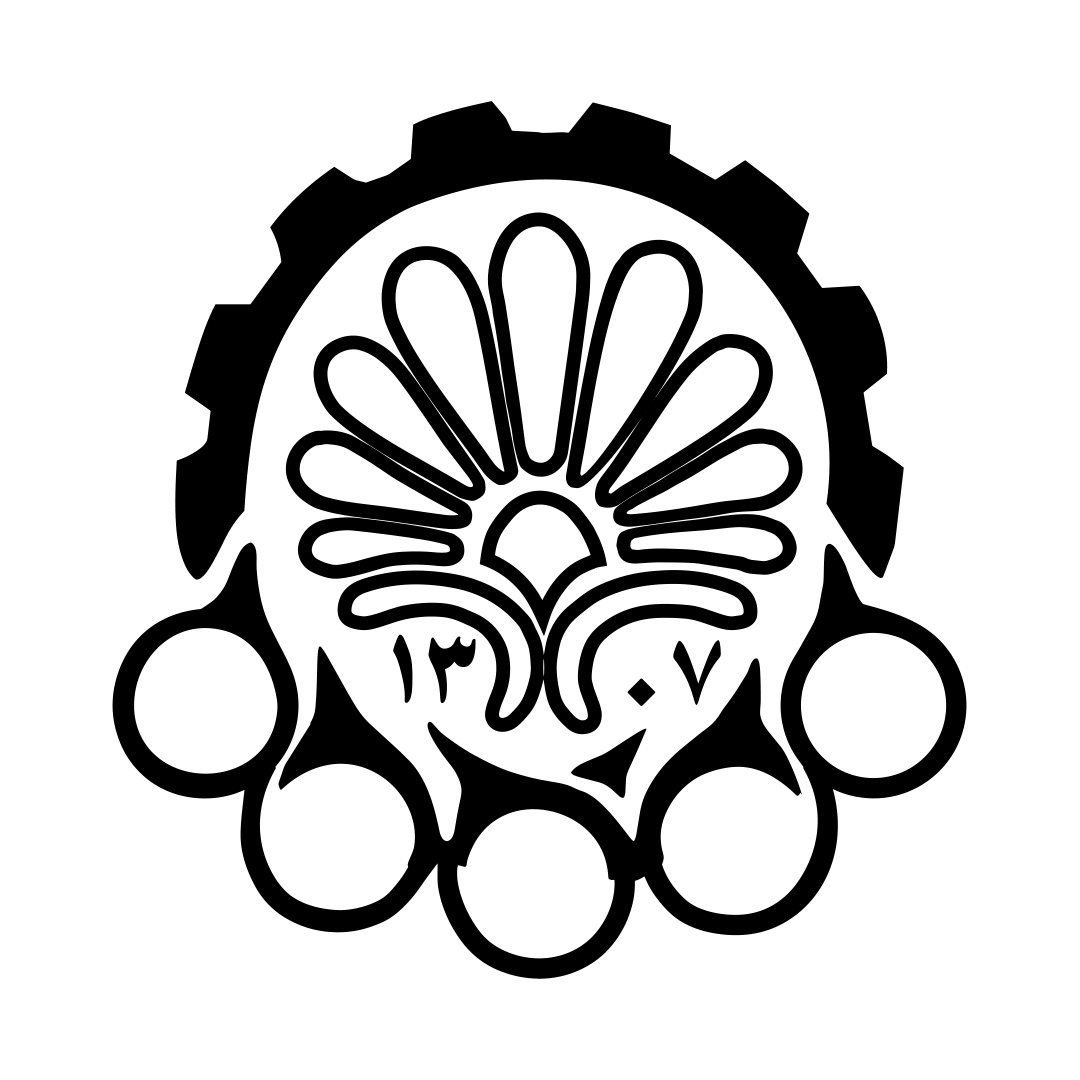
\includegraphics[width=44mm]{assets/aut-logo-black.png}\par
    \vspace{3mm}

    {\Large\bfseries \universityname\par}
    \vspace{1mm}
    {\large (\universityalias)\par}
    \vspace{1mm}
    {\large \facultyname\par}

    \vspace{8mm}
    {\Large\bfseries درس \coursename\par}

    \vspace{12mm}
    {\large عنوان\par}
    \vspace{2mm}
    {\LARGE\bfseries تمرین شماره \assignmentnumber\par}

    \vspace{10mm}
    {\large تهیه‌کننده\par}
    \vspace{2mm}
    {\Large\bfseries \studentname\par}

    \vspace{10mm}
    {\large استاد درس\par}
    \vspace{2mm}
    {\Large\bfseries \instructorname\par}

    \vspace{10mm}
    {\Large \assignmentdate\par}
    \vfill
  \end{titlepage}
  \setcounter{page}{1}%
}


\XeTeXgenerateactualtext=1
\newcommand{\exnum}[1]{\mbox{\beginL#1\endL}}
\renewcommand{\exercise}[1]{\clearpage\section*{تمرین \exnum{#1}}}
\setlength{\emergencystretch}{3em}
\allowdisplaybreaks[1]
\hypersetup{pdftitle={تمرینات فصل دو (سری دوم)},pdfauthor={محمد خلیلی اصل}}
% Use the shared cover with the user-specified assignment title.
\AssignmentNumber{تمرینات فصل دو (سری دوم)}
\AssignmentDate{مهلت: ۲۷ آبان ۱۴۰۵}
% etoolbox is already loaded by the shared siunitx dependency.
\patchcmd{\MakeAssignmentCover}{تمرین شماره \assignmentnumber}{\assignmentnumber}{}{\errmessage{Cover title replacement failed}}
\begin{document}
\MakeAssignmentCover
% !TeX root = ../main.tex
\exercise{۲.۱۶}\label{sec:ex16}

\subsection*{صورت مسئله و فرض‌ها}

صورت تمرین در صفحه چاپی ۹۷ کتاب، استخراج \(V_{\mathrm{out}}\) برحسب \(V_{\mathrm{in}}\) را برای نواحی \lr{B} و \lr{D} اینورتر \lr{CMOS} با \(\beta_n=\beta_p\) و \(V_{tn}=|V_{tp}|\) می‌خواهد \cite{weste}. در این پاسخ، مطابق تحلیل بخش \exnum{۲.۵.۱}، از مدل \lr{Long-channel} یا \lr{Shockley} استفاده می‌کنیم. فرض‌ها عبارت‌اند از:

\begin{itemize}
\item \(V_{tn}=|V_{tp}|=V_t>0\)، \(\beta_n=\beta_p=\beta>0\) و \(V_{\mathrm{DD}}>2V_t\)؛ شرط آخر وجود بازه هم‌زمان روشن‌بودن دو ترانزیستور را تضمین می‌کند.
\item \lr{Channel-length Modulation} و \lr{Leakage} در مدل منظور نمی‌شوند.
\item بدنه \lr{nMOS} به زمین و بدنه \lr{pMOS} به \(V_{\mathrm{DD}}\) متصل است؛ بنابراین در این اینورتر \(V_{\mathrm{SB}}=0\) است.
\item تحلیل \lr{DC} است و خروجی جریان بار \lr{DC} ندارد؛ در نتیجه، \lr{KCL} در گره خروجی به \(I_{dsn}=|I_{dsp}|\) می‌انجامد \cite[بخش \exnum{۲.۵.۱}]{weste} و \cite[اسلاید ۳]{dcslides}.
\end{itemize}

پارامتر \(\beta=\mu C_{\mathrm{ox}}W/L\) ضریب جریان است. برابری \(\beta_n\) و \(\beta_p\) به معنی برابری ابعاد دو ترانزیستور نیست؛ تفاوت \lr{Mobility} معمولاً با انتخاب نسبت ابعاد مناسب جبران می‌شود \cite[صفحه چاپی ۸۸]{weste}.

ولتاژهای مورد استفاده در روابط جریان چنین‌اند:

\nopagebreak[3]
\begin{equation}\label{eq:ex16-1}
V_{gsn}=V_{\mathrm{in}},\qquad V_{dsn}=V_{\mathrm{out}},
\end{equation}
\nopagebreak[3]
\begin{equation}\label{eq:ex16-2}
V_{sgp}=V_{\mathrm{DD}}-V_{\mathrm{in}},\qquad
V_{sdp}=V_{\mathrm{DD}}-V_{\mathrm{out}}.
\end{equation}

استفاده از \(V_{sgp}\) و \(V_{sdp}\) مثبت، علامت جریان \lr{pMOS} را از اندازه آن جدا می‌کند.

\subsection*{ناحیه \lr{B}: \lr{nMOS} در \lr{Saturation} و \lr{pMOS} در \lr{Linear}}

درون این ناحیه، \(V_t<V_{\mathrm{in}}<V_{\mathrm{DD}}/2\) است. شرایط \lr{Operating Region} عبارت‌اند از \(V_{\mathrm{out}}\ge V_{\mathrm{in}}-V_t\) برای \lr{nMOS} و \(V_{\mathrm{out}}>V_{\mathrm{in}}+V_t\) برای \lr{pMOS} \cite[جدول‌های \exnum{۲.۲} و \exnum{۲.۳}]{weste} و \cite[اسلایدهای ۵ تا ۷]{dcslides}. برابری جریان‌ها در مدل \lr{Shockley} می‌دهد:

\nopagebreak[3]
\begin{equation}\label{eq:ex16-3}
\frac{\beta}{2}(V_{\mathrm{in}}-V_t)^2
=\beta\left[
(V_{\mathrm{DD}}-V_{\mathrm{in}}-V_t)(V_{\mathrm{DD}}-V_{\mathrm{out}})
-\frac{(V_{\mathrm{DD}}-V_{\mathrm{out}})^2}{2}
\right].
\end{equation}

با تعریف \(Y=V_{\mathrm{DD}}-V_{\mathrm{out}}\)، معادله درجه دوم زیر به دست می‌آید:

\nopagebreak[3]
\begin{equation}\label{eq:ex16-4}
Y^2-2(V_{\mathrm{DD}}-V_{\mathrm{in}}-V_t)Y
+(V_{\mathrm{in}}-V_t)^2=0.
\end{equation}

دو ریشه این معادله عبارت‌اند از:

\nopagebreak[3]
\begin{equation}\label{eq:ex16-5}
Y=V_{\mathrm{DD}}-V_{\mathrm{in}}-V_t
\pm\sqrt{(V_{\mathrm{DD}}-V_{\mathrm{in}}-V_t)^2-(V_{\mathrm{in}}-V_t)^2}.
\end{equation}

شرط \lr{Linear} بودن \lr{pMOS}، یعنی \(Y<V_{\mathrm{DD}}-V_{\mathrm{in}}-V_t\)، ریشه دارای علامت منفی را انتخاب می‌کند. با استفاده از همانی تفاضل دو مربع، نتیجه نهایی چنین است:

\nopagebreak[3]
\begin{equation}\label{eq:ex16-6}
\boxed{
V_{\mathrm{out}}
=V_{\mathrm{in}}+V_t
+\sqrt{(V_{\mathrm{DD}}-2V_{\mathrm{in}})(V_{\mathrm{DD}}-2V_t)}
}.
\end{equation}

در بازه مشخص‌شده، عبارت زیر رادیکال مثبت است؛ بنابراین \(V_{\mathrm{out}}>V_{\mathrm{in}}+V_t\) و هر دو شرط \lr{Operating Region} برقرارند. همچنین، با \(a=V_{\mathrm{in}}-V_t\) و \(b=V_{\mathrm{DD}}-V_{\mathrm{in}}-V_t\)، داریم \(0<a<b\) و \(Y=b-\sqrt{b^2-a^2}\in(0,b)\)؛ پس خروجی از محدوده تغذیه خارج نمی‌شود.

در مرز \(V_{\mathrm{in}}=V_t\)، رابطه به \(V_{\mathrm{out}}=V_{\mathrm{DD}}\) می‌رسد؛ این نقطه مرز \lr{Cutoff} و روشن‌شدن \lr{nMOS} است. حد یک‌طرفه خروجی در مرز ناحیه \lr{C} نیز برابر است با:

\nopagebreak[3]
\begin{equation}\label{eq:ex16-7}
\lim_{V_{\mathrm{in}}\to(V_{\mathrm{DD}}/2)^-}V_{\mathrm{out}}
=\frac{V_{\mathrm{DD}}}{2}+V_t.
\end{equation}

\subsection*{ناحیه \lr{D}: \lr{nMOS} در \lr{Linear} و \lr{pMOS} در \lr{Saturation}}

درون این ناحیه، \(V_{\mathrm{DD}}/2<V_{\mathrm{in}}<V_{\mathrm{DD}}-V_t\) است. شرایط \lr{Operating Region} عبارت‌اند از \(V_{\mathrm{out}}<V_{\mathrm{in}}-V_t\) برای \lr{nMOS} و \(V_{\mathrm{out}}\le V_{\mathrm{in}}+V_t\) برای \lr{pMOS} \cite[جدول‌های \exnum{۲.۲} و \exnum{۲.۳}]{weste}. از برابری جریان‌ها داریم:

\nopagebreak[3]
\begin{equation}\label{eq:ex16-8}
\beta\left[(V_{\mathrm{in}}-V_t)V_{\mathrm{out}}
-\frac{V_{\mathrm{out}}^2}{2}\right]
=\frac{\beta}{2}(V_{\mathrm{DD}}-V_{\mathrm{in}}-V_t)^2.
\end{equation}

مرتب‌کردن این رابطه می‌دهد:

\nopagebreak[3]
\begin{equation}\label{eq:ex16-9}
V_{\mathrm{out}}^2-2(V_{\mathrm{in}}-V_t)V_{\mathrm{out}}
+(V_{\mathrm{DD}}-V_{\mathrm{in}}-V_t)^2=0.
\end{equation}

برای رعایت شرط \lr{Linear} بودن \lr{nMOS}، باید ریشه کوچک‌تر انتخاب شود. بنابراین:

\nopagebreak[3]
\begin{equation}\label{eq:ex16-10}
\boxed{
V_{\mathrm{out}}
=V_{\mathrm{in}}-V_t
-\sqrt{(2V_{\mathrm{in}}-V_{\mathrm{DD}})(V_{\mathrm{DD}}-2V_t)}
}.
\end{equation}

با \(a=V_{\mathrm{in}}-V_t\) و \(b=V_{\mathrm{DD}}-V_{\mathrm{in}}-V_t\)، درون این ناحیه \(0<b<a\) و \(V_{\mathrm{out}}=a-\sqrt{a^2-b^2}\in(0,a)\) است. پس خروجی نامنفی است و هر دو شرط \lr{Operating Region} برقرارند.

در مرز \(V_{\mathrm{in}}=V_{\mathrm{DD}}-V_t\)، خروجی صفر ولت می‌شود. حد یک‌طرفه در مرز دیگر نیز برابر است با:

\nopagebreak[3]
\begin{equation}\label{eq:ex16-11}
\lim_{V_{\mathrm{in}}\to(V_{\mathrm{DD}}/2)^+}V_{\mathrm{out}}
=\frac{V_{\mathrm{DD}}}{2}-V_t.
\end{equation}

\subsection*{تفسیر ناحیه \lr{C} و کنترل تقارن}

در \(V_{\mathrm{in}}=V_{\mathrm{DD}}/2\)، هر دو ترانزیستور در \lr{Saturation} قرار دارند و جریان‌های مدل ایدئال برای هر خروجی در بازه زیر برابرند:

\nopagebreak[3]
\begin{equation}\label{eq:ex16-12}
\frac{V_{\mathrm{DD}}}{2}-V_t
\le V_{\mathrm{out}}\le
\frac{V_{\mathrm{DD}}}{2}+V_t.
\end{equation}

بنابراین، مدل \lr{DC} ایدئال در این ورودی، خروجی یکتایی تعیین نمی‌کند. دو حد محاسبه‌شده، انتهای بالایی و پایینی این پاره‌خط عمودی‌اند؛ نسبت‌دادن یک خروجی یکتا به کل ناحیه \lr{C} دقیق نیست. \lr{Channel-length Modulation} در ترانزیستور واقعی، شیب انتقال را محدود می‌کند \cite[صفحه چاپی ۸۸]{weste}.

دو شاخه به‌دست‌آمده در روابط~\eqref{eq:ex16-6} و~\eqref{eq:ex16-10} تقارن مورد انتظار را نیز دارند:

\nopagebreak[3]
\begin{equation}\label{eq:ex16-13}
V_{\mathrm{out,D}}(V_{\mathrm{DD}}-V_{\mathrm{in}})
=V_{\mathrm{DD}}-V_{\mathrm{out,B}}(V_{\mathrm{in}}).
\end{equation}

این رابطه یک کنترل مستقل برای علامت رادیکال و سازگاری دو جواب است.


% !TeX root = ../main.tex
\exercise{۲.۱۷}\label{sec:ex17}

\subsection*{صورت مسئله و تعریف سطوح منطقی}

طبق صورت تمرین، \(V_{\mathrm{DD}}=\qty{1.0}{\volt}\)، \(V_{tn}=|V_{tp}|=V_t=\qty{0.35}{\volt}\) و \(\beta_n=\beta_p\) است \cite[صفحه چاپی ۹۷]{weste}. مدل و شرایط تحلیل همان فرض‌های تمرین \exnum{۲.۱۶} هستند؛ شرط \(V_{\mathrm{DD}}>2V_t\) نیز برقرار است. برابری \(\beta\) بیانگر برابری ضریب جریان است و برابری ابعاد \lr{nMOS} و \lr{pMOS} را الزام نمی‌کند.

مطابق تعریف کتاب و اسلایدها، \(V_{\mathrm{IL}}\) و \(V_{\mathrm{IH}}\) در دو نقطه \lr{Unity Gain} با شیب \(-1\) تعیین می‌شوند. حداقل خروجی \lr{HIGH} و حداکثر خروجی \lr{LOW} متناظر با بدترین ورودی‌های مجاز عبارت‌اند از \cite[بخش \exnum{۲.۵.۳}]{weste} و \cite[اسلایدهای ۹ و ۱۰]{dcslides}:

\nopagebreak[3]
\begin{equation}\label{eq:ex17-1}
V_{\mathrm{OH}}=V_{\mathrm{out}}(V_{\mathrm{IL}}),\qquad
V_{\mathrm{OL}}=V_{\mathrm{out}}(V_{\mathrm{IH}}).
\end{equation}

بنابراین، تعریف \lr{Noise Margin} برای این سطوح چنین است:

\nopagebreak[3]
\begin{equation}\label{eq:ex17-2}
NM_{\mathrm{L}}=V_{\mathrm{IL}}-V_{\mathrm{OL}},\qquad
NM_{\mathrm{H}}=V_{\mathrm{OH}}-V_{\mathrm{IH}}.
\end{equation}

مقادیر \(V_{\mathrm{OH}}\) و \(V_{\mathrm{OL}}\) در این تعریف، به‌ترتیب با \(V_{\mathrm{DD}}\) و صفر جایگزین نمی‌شوند؛ ورودیِ نزدیک مرز مجاز، اندکی افت خروجی ایجاد می‌کند.

\subsection*{استخراج نقاط \lr{Unity Gain}}

از رابطه~\eqref{eq:ex16-6} برای شاخه \lr{B} در تمرین \exnum{۲.۱۶}، مشتق خروجی برابر است با:

\nopagebreak[3]
\begin{equation}\label{eq:ex17-3}
\frac{dV_{\mathrm{out}}}{dV_{\mathrm{in}}}
=1-\sqrt{\frac{V_{\mathrm{DD}}-2V_t}{V_{\mathrm{DD}}-2V_{\mathrm{in}}}}.
\end{equation}

با قرار دادن مشتق برابر \(-1\) در \(V_{\mathrm{in}}=V_{\mathrm{IL}}\)، ریشه مثبت باید برابر ۲ باشد. در نتیجه:

\nopagebreak[3]
\begin{equation}\label{eq:ex17-4}
V_{\mathrm{DD}}-2V_{\mathrm{IL}}
=\frac{V_{\mathrm{DD}}-2V_t}{4},
\qquad
\boxed{V_{\mathrm{IL}}=\frac{3V_{\mathrm{DD}}+2V_t}{8}}.
\end{equation}

برای شاخه \lr{D} نیز داریم:

\nopagebreak[3]
\begin{equation}\label{eq:ex17-5}
\frac{dV_{\mathrm{out}}}{dV_{\mathrm{in}}}
=1-\sqrt{\frac{V_{\mathrm{DD}}-2V_t}{2V_{\mathrm{in}}-V_{\mathrm{DD}}}}.
\end{equation}

اعمال شرط شیب \(-1\) در \(V_{\mathrm{in}}=V_{\mathrm{IH}}\) می‌دهد:

\nopagebreak[3]
\begin{equation}\label{eq:ex17-6}
2V_{\mathrm{IH}}-V_{\mathrm{DD}}
=\frac{V_{\mathrm{DD}}-2V_t}{4},
\qquad
\boxed{V_{\mathrm{IH}}=\frac{5V_{\mathrm{DD}}-2V_t}{8}}.
\end{equation}

اعتبار استفاده از شاخه‌های \lr{B} و \lr{D} را می‌توان مستقیماً بررسی کرد:

\nopagebreak[3]
\begin{equation}\label{eq:ex17-7}
V_{\mathrm{IL}}-V_t
=V_{\mathrm{DD}}-V_t-V_{\mathrm{IH}}
=\frac{3(V_{\mathrm{DD}}-2V_t)}{8}>0,
\end{equation}
\nopagebreak[3]
\begin{equation}\label{eq:ex17-8}
\frac{V_{\mathrm{DD}}}{2}-V_{\mathrm{IL}}
=V_{\mathrm{IH}}-\frac{V_{\mathrm{DD}}}{2}
=\frac{V_{\mathrm{DD}}-2V_t}{8}>0.
\end{equation}

پس دو نقطه درون نواحی فرض‌شده قرار دارند و از مرز عمودی ناحیه \lr{C} جدا هستند.

\subsection*{استخراج سطوح خروجی و \lr{Noise Margin}}

در دو نقطه \lr{Unity Gain}، مقدار رادیکالِ رابطه خروجی برابر \((V_{\mathrm{DD}}-2V_t)/2\) است. جایگذاری آن در شاخه‌های \lr{B} و \lr{D} می‌دهد:

\nopagebreak[3]
\begin{equation}\label{eq:ex17-9}
V_{\mathrm{OH}}
=V_{\mathrm{IL}}+V_t+\frac{V_{\mathrm{DD}}-2V_t}{2}
=\frac{7V_{\mathrm{DD}}+2V_t}{8},
\end{equation}
\nopagebreak[3]
\begin{equation}\label{eq:ex17-10}
V_{\mathrm{OL}}
=V_{\mathrm{IH}}-V_t-\frac{V_{\mathrm{DD}}-2V_t}{2}
=\frac{V_{\mathrm{DD}}-2V_t}{8}.
\end{equation}

بنابراین، حاشیه‌های بالا و پایین برابرند:

\nopagebreak[3]
\begin{equation}\label{eq:ex17-11}
\boxed{
NM_{\mathrm{L}}=NM_{\mathrm{H}}
=\frac{V_{\mathrm{DD}}+2V_t}{4}
}.
\end{equation}

این برابری از تقارن \lr{VTC} ناشی می‌شود و با \(V_{\mathrm{IL}}+V_{\mathrm{IH}}=V_{\mathrm{DD}}\) و \(V_{\mathrm{OL}}+V_{\mathrm{OH}}=V_{\mathrm{DD}}\) نیز سازگار است.

\clearpage
\subsection*{نتایج عددی و شیوه گزارش}

با جایگذاری داده‌های مسئله، مقادیر جدول~\ref{tab:noise} حاصل می‌شوند. ارقام اعشاری برای امکان بازبینی محاسبات مدل حفظ شده‌اند و بیانگر دقت فیزیکی یک فناوری واقعی نیستند.

\begin{table}[htbp]\centering
\caption{نتایج محاسبات سطوح منطقی و حاشیه نویز}
\label{tab:noise}
\begin{tabularx}{\linewidth}{ccX}\toprule
کمیت & رابطه تحلیلی & مقدار محاسباتی در مدل\\
\midrule
\(V_{\mathrm{IL}}\) & \((3V_{\mathrm{DD}}+2V_t)/8\) & \(\qty{0.4625}{\volt}\)\\
\(V_{\mathrm{IH}}\) & \((5V_{\mathrm{DD}}-2V_t)/8\) & \(\qty{0.5375}{\volt}\)\\
\(V_{\mathrm{OL}}\) & \((V_{\mathrm{DD}}-2V_t)/8\) & \(\qty{0.0375}{\volt}\)\\
\(V_{\mathrm{OH}}\) & \((7V_{\mathrm{DD}}+2V_t)/8\) & \(\qty{0.9625}{\volt}\)\\
\(NM_{\mathrm{L}}\) & \((V_{\mathrm{DD}}+2V_t)/4\) & \(\qty{0.425}{\volt}\)\\
\(NM_{\mathrm{H}}\) & \((V_{\mathrm{DD}}+2V_t)/4\) & \(\qty{0.425}{\volt}\)\\
\bottomrule\end{tabularx}\end{table}

پس پاسخ نهایی در مدل مسئله چنین است:

\nopagebreak[3]
\begin{equation}\label{eq:ex17-12}
\boxed{NM_{\mathrm{L}}=NM_{\mathrm{H}}=\qty{0.425}{\volt}
=0.425V_{\mathrm{DD}}}.
\end{equation}

این مقدار برابر \num{42.5} درصد ولتاژ تغذیه است. در صورت نیاز به گزارش با دو رقم اعشار و با قاعده گردکردن نیم‌به‌بالا، مقدار \(\qty{0.43}{\volt}\) گزارش می‌شود.

در \lr{Solutions}، چهار سطح ولتاژ به‌صورت \(0.46\)، \(0.54\)، \(0.04\) و \(\qty{0.96}{\volt}\) و حاشیه‌ها به‌صورت \(\qty{0.42}{\volt}\) گزارش شده‌اند \cite[صفحات ۵ و ۶]{manual}. تفاضل سطوح خروجی و ورودیِ ازپیش‌گردشده نیز همین مقدار اخیر را می‌دهد. روش تقریب در آن منبع تصریح نشده است. برای جلوگیری از خطای گردکردن میانی، پاسخ اصلی اینجا همان \(\qty{0.425}{\volt}\) باقی می‌ماند.


% !TeX root = ../main.tex
\exercise{۲.۲۰}\label{sec:ex20}

\subsection*{صورت مسئله و محدوده مدل}

هدف، تعیین ولتاژ خروجی چهار مدار شکل \exnum{۲.۳۵} کتاب با صرف‌نظر از \lr{Body Effect} است \cite[صفحه چاپی ۹۷]{weste}. اتصال‌ها مستقیماً با شکل کتاب تطبیق داده شده‌اند. خط افقی تغذیه در شکل نشان‌دهنده \(V_{\mathrm{DD}}\)، نماد زمین نشان‌دهنده صفر ولت و حباب \lr{Gate} مشخص‌کننده \lr{pMOS} است.

مطابق تحلیل \lr{Threshold Drop} کتاب، از مدل \lr{Cutoff} با آستانه ثابت، بدون جریان بار \lr{DC} و بدون \lr{Leakage} استفاده می‌کنیم \cite[بخش \exnum{۲.۵.۴}]{weste} و \cite[اسلاید ۱۲]{dcslides}. منظور از خروجی‌های دارای افت، حد شارژ یا دشارژ در این مدل ساده است. این پاسخ بر رسیدن گره‌ها از سمت قابل‌هدایت به حد موردنظر تکیه دارد؛ برای گره شناور با شرایط اولیه دلخواه، الزاماً یک نقطه \lr{DC} یکتا وجود ندارد. کتاب نیز در پانوشت صفحه چاپی ۹۲، تغییر بسیار آهسته خروجی بر اثر \lr{Subthreshold Leakage} را یادآوری می‌کند.

برای نتایج متعارف زیر، تغذیه باید امکان روشن‌شدن ترانزیستورهای مربوط را بدهد: در بخش \lr{(b)}، \(V_{\mathrm{DD}}>2|V_{tp}|\) و در بخش \lr{(c)}، \(V_{\mathrm{DD}}>|V_{tp}|+V_{tn}\) فرض می‌شود. این‌ها شرط اعتبار تحلیل‌اند و داده عددی تازه‌ای برای مسئله نیستند.

\subsection*{قواعد انتقال ولتاژ}

در \lr{nMOS}، پایانه دارای ولتاژ کمتر نقش \lr{Source} را دارد. ترانزیستور با \(V_{gs}>V_{tn}\) هدایت می‌کند. بنابراین با \lr{Gate} در \(V_{\mathrm{DD}}\)، صفر را بدون افت آستانه عبور می‌دهد و هنگام شارژ یک گره از ولتاژ پایین، حد بالای آن برابر است با:

\nopagebreak[3]
\begin{equation}\label{eq:ex20-1}
V_{\mathrm{out,lim}}=V_g-V_{tn}=V_{\mathrm{DD}}-V_{tn}.
\end{equation}

در \lr{pMOS}، پایانه دارای ولتاژ بیشتر نقش \lr{Source} را دارد. شرط هدایت \(V_{sg}>|V_{tp}|\) است. این ترانزیستور با \lr{Gate} صفر، سطح \lr{HIGH} را بدون افت آستانه عبور می‌دهد؛ هنگام دشارژ یک گره به سمت زمین، حد پایین هدایت برابر است با:

\nopagebreak[3]
\begin{equation}\label{eq:ex20-2}
V_{\mathrm{out,lim}}=V_g+|V_{tp}|.
\end{equation}

در مرز آستانه، جریان مدل ایدئال به صفر می‌رسد. ازاین‌رو، برابری در دو رابطه بالا حد هدایت را مشخص می‌کند \cite[صفحات چاپی ۹۲ و ۹۳]{weste}.

\clearpage
\subsection*{تحلیل چهار مدار}

\subsubsection*{مدار \lr{(a)}: دو \lr{nMOS} در مسیر زمین}

ورودی ترانزیستور نخست زمین است و \lr{Gate} هر دو \lr{nMOS} به \(V_{\mathrm{DD}}\) متصل است. ترانزیستور نخست گره میانی را به صفر می‌رساند و ترانزیستور دوم نیز همان صفر را به خروجی منتقل می‌کند. با \(V_{\mathrm{DD}}>V_{tn}\)، مسیر دشارژ تا صفر هدایت دارد؛ در نتیجه:

\nopagebreak[3]
\begin{equation}\label{eq:ex20-3}
\boxed{V_{\mathrm{out}}=\qty{0}{\volt}}.
\end{equation}

سری‌شدن این دو ترانزیستور افت آستانه‌ای به سطح \lr{LOW} اضافه نمی‌کند؛ البته بر جریان و زمان دشارژ اثر می‌گذارد.

\subsubsection*{مدار \lr{(b)}: خروجی \lr{pMOS} نخست متصل به \lr{Gate} ترانزیستور دوم}

دو ترانزیستور در این مدار در یک مسیر \lr{Source–Drain} سری قرار ندارند. پایانه چپ و \lr{Gate} ترانزیستور نخست زمین‌اند؛ پایانه راست آن، گره \(X\)، به \lr{Gate} ترانزیستور دوم متصل است. پایانه چپ ترانزیستور دوم نیز زمین است و پایانه راست آن خروجی مدار را تشکیل می‌دهد.

هنگام دشارژ گره \(X\) از ولتاژ بالاتر، شرط هدایت ترانزیستور نخست \(V_X>|V_{tp}|\) است؛ بنابراین حد دشارژ برابر است با:

\nopagebreak[3]
\begin{equation}\label{eq:ex20-4}
V_{X,\mathrm{lim}}=|V_{tp}|.
\end{equation}

اگر خروجی ترانزیستور دوم از ولتاژ بالاتر دشارژ شود، شرط هدایت آن \(V_{\mathrm{out}}-V_X>|V_{tp}|\) خواهد بود. با رسیدن گره \(X\) به حد یادشده، حد دشارژ خروجی چنین است:

\nopagebreak[3]
\begin{equation}\label{eq:ex20-5}
\boxed{V_{\mathrm{out,lim}}=V_X+|V_{tp}|=2|V_{tp}|}.
\end{equation}

افت اضافی از کنترل \lr{Gate} دوم با یک سطح \lr{LOW} تضعیف‌شده ناشی می‌شود. اگر گره \(X\) از ابتدا زیر حد آستانه باشد، مدل بدون \lr{Leakage} آن را به \(|V_{tp}|\) شارژ نمی‌کند؛ بنابراین مقدار فوق را نباید مستقل از شرایط اولیه دلخواه، یک خروجی \lr{DC} تضمین‌شده دانست.

\subsubsection*{مدار \lr{(c)}: \lr{pMOS} و \lr{nMOS} در مسیر زمین}

\lr{Gate} ترانزیستور \lr{pMOS} نخست صفر است و ورودی آن نیز به زمین متصل است. گره میانی \(X\) در دشارژ از ولتاژ بالاتر تا حد زیر پایین می‌آید:

\nopagebreak[3]
\begin{equation}\label{eq:ex20-6}
V_{X,\mathrm{lim}}=|V_{tp}|.
\end{equation}

\lr{Gate} ترانزیستور \lr{nMOS} دوم به \(V_{\mathrm{DD}}\) متصل است. با شرط \(V_{\mathrm{DD}}-|V_{tp}|>V_{tn}\)، این ترانزیستور در حوالی حد نهایی همچنان هدایت دارد و دو گره میانی و خروجی را هم‌ولتاژ می‌کند. پس:

\nopagebreak[3]
\begin{equation}\label{eq:ex20-7}
\boxed{V_{\mathrm{out,lim}}=|V_{tp}|}.
\end{equation}

در این مدار، \lr{nMOS} افت آستانه تازه‌ای به مقدار \lr{LOW} تضعیف‌شده اضافه نمی‌کند. در مدل بدون \lr{Leakage}، شرط اولیه گره‌ها همچنان در تعبیر حد دشارژ اهمیت دارد.

\subsubsection*{مدار \lr{(d)}: \lr{pMOS} و \lr{nMOS} در مسیر تغذیه}

ورودی \lr{pMOS} برابر \(V_{\mathrm{DD}}\) و \lr{Gate} آن صفر است. با \(V_{\mathrm{DD}}>|V_{tp}|\)، گره میانی به \(V_{\mathrm{DD}}\) شارژ می‌شود. \lr{nMOS} دوم نیز \lr{Gate} با ولتاژ \(V_{\mathrm{DD}}\) دارد؛ هنگام شارژ خروجی از سطح پایین، با افزایش خروجی، \(V_{gs}\) کاهش می‌یابد. در مرز \(V_{gs}=V_{tn}\)، جریان مدل به صفر می‌رسد و داریم:

\nopagebreak[3]
\begin{equation}\label{eq:ex20-8}
\boxed{V_{\mathrm{out,lim}}=V_{\mathrm{DD}}-V_{tn}}.
\end{equation}

در نتیجه، انتقال \lr{HIGH} توسط \lr{pMOS} افتی ایجاد نمی‌کند و افت نهایی از \lr{nMOS} ناشی می‌شود.

\subsection*{جمع‌بندی و تفسیر}

جدول~\ref{tab:pass} پاسخ متعارف مسئله در مدل \lr{Threshold Drop} و با شرایط شارژ یا دشارژ بیان‌شده را خلاصه می‌کند.

\begin{table}[htbp]\centering
\caption{خروجی شبکه‌های ترانزیستوری}
\label{tab:pass}
\begin{tabularx}{\linewidth}{ccX}\toprule
مدار & خروجی یا حد انتقال & علت\\
\midrule
\lr{(a)} & \(\qty{0}{\volt}\) & انتقال \lr{LOW} توسط دو \lr{nMOS}\\
\lr{(b)} & \(2|V_{tp}|\) & \lr{LOW} تضعیف‌شده در \lr{Gate} ترانزیستور \lr{pMOS} دوم\\
\lr{(c)} & \(|V_{tp}|\) & افت ناشی از \lr{pMOS} نخست و هدایت \lr{nMOS} دوم\\
\lr{(d)} & \(V_{\mathrm{DD}}-V_{tn}\) & محدودیت شارژ خروجی توسط \lr{nMOS}\\
\bottomrule\end{tabularx}\end{table}

نتیجه بخش \lr{(b)} با سری‌کردن ساده دو \lr{pMOS} در مسیر عبور سیگنال یکسان نیست. تفاوت اتصال \lr{Gate} و مسیر \lr{Source–Drain}، علت انباشته‌شدن افت در آن مدار است؛ این تمایز در بخش \exnum{۲.۵.۴} کتاب نیز توضیح داده شده است. این نتایج، پیش‌بینی مدل ساده تمرین‌اند و شامل محاسبه \lr{Leakage}، زمان نشست یا شبیه‌سازی یک فناوری واقعی نمی‌شوند.


\clearpage
\begin{thebibliography}{9}
\bibitem{weste}
\lr{Neil H. E. Weste and David Money Harris}،
\lr{CMOS VLSI Design: A Circuits and Systems Perspective}،
ویرایش چهارم، \lr{Addison-Wesley (Pearson Education)}، ۲۰۱۱.
صورت تمرین‌ها و شکل \exnum{۲.۳۵}: صفحه چاپی ۹۷، صفحه ۱۲۴ فایل \lr{PDF}.
تحلیل اینورتر: بخش \exnum{۲.۵.۱}، صفحات چاپی ۸۸ و ۸۹؛
\lr{Noise Margin}: بخش \exnum{۲.۵.۳}، صفحات چاپی ۹۱ و ۹۲؛
\lr{Pass Transistor}: بخش \exnum{۲.۵.۴}، صفحات چاپی ۹۲ و ۹۳.
در این بخش‌ها شماره صفحه فایل برابر شماره چاپی به‌اضافه ۲۷ است.
\bibitem{dcslides}
\lr{CMOS Inverter DC Characteristics}، اسلایدهای درس در مجموعه اسلایدهای
\lr{CMOS VLSI Design, Fourth Edition}، برگرفته از یادداشت‌های
\lr{David Money Harris} (۲۰۱۱).
تحلیل اینورتر: اسلایدهای ۳ تا ۷؛ سطوح منطقی و نویز: ۹ و ۱۰؛
\lr{Pass Transistor}: ۱۲ و ۱۳؛ فهرست تمرین‌ها: ۱۴.
شماره اسلاید و صفحه فایل یکسان‌اند.
\bibitem{manual}
\lr{Solutions}، پاسخ‌های تمرین‌ها، با شناسه داخلی \lr{Version 2.0 completed 12/23/04}.
فصل ۲، پاسخ \exnum{۲.۱۷}، صفحات ۵ و ۶.
نام پدیدآورنده و ویرایش کتابِ مبنای این مجموعه احراز نشده‌اند.
این پاسخ پس از تطبیق داده‌ها و محاسبه مستقل، فقط برای کنترل جانبی استفاده شده است.
\end{thebibliography}
\end{document}
